\newpage

\section{Moments d'une distribution}

\subsection{Définitions fondamentales des moments}

Après avoir défini l'espérance ($\mu$) et la variance ($\sigma^2$), qui sont les moments d'ordre 1 et 2, nous pouvons généraliser cette idée pour capturer des informations plus subtiles sur la forme d'une distribution.

\begin{definitionbox}[Types de Moments]
Soit $X$ une variable aléatoire ayant une espérance $\mu$ et une variance $\sigma^2$. Pour tout entier positif $m$, on définit les moments suivants :
\begin{itemize}
    \item \textbf{$m$-ième moment (non centré)} : $E[X^m]$.
    \item \textbf{$m$-ième moment centré} : $E[(X - \mu)^m]$.
    \item \textbf{$m$-ième moment standardisé} : $E\left[\left(\frac{X - \mu}{\sigma}\right)^m\right]$.
\end{itemize}
Les moments centrés et standardisés permettent d'étudier les propriétés de la distribution indépendamment de sa position ($\mu$) et de son échelle ($\sigma$).
\end{definitionbox}

\subsection{Asymétrie (Skewness)}

Le premier moment nous donne la tendance centrale. Le deuxième moment (la variance) nous donne la dispersion. Le troisième moment, lui, va nous renseigner sur la \textit{symétrie} de la distribution.

\begin{definitionbox}[Asymétrie (Skewness)]
L'\textbf{asymétrie} (ou \textit{skewness}) d'une variable aléatoire $X$ de moyenne $\mu$ et d'écart-type $\sigma$ est définie comme le \textbf{troisième moment standardisé} :
$$ \text{Skew}(X) = E\left[ \left( \frac{X - \mu}{\sigma} \right)^3 \right]. $$
\end{definitionbox}

\begin{intuitionbox}[Comprendre la Formule du Skewness]
Pour une variable aléatoire $X$ de moyenne $\mu$ et d'écart-type $\sigma$, le \textbf{skewness} est défini comme :
\[
\text{Skew}(X) = \frac{E[(X - \mu)^3]}{\sigma^3}
\]

\medskip

\textbf{Logique du numérateur : le moment centré d'ordre 3}
\begin{itemize}
    \item Le terme $(X - \mu)^3$ est le \textbf{cube de l'écart à la moyenne}
    \item Contrairement à $(X - \mu)^2$ (toujours positif), le cube \textbf{conserve le signe} de l'écart
    \item Il pondère différemment les observations à gauche et à droite de la moyenne
\end{itemize}

\medskip

% --- MODIFIÉ : Tableau supprimé et fusionné dans la liste ---
\textbf{Interprétation intuitive}
\begin{itemize}
    \item \textbf{Skewness = 0 (Symétrique)} : La distribution est symétrique. Les écarts positifs et négatifs s'annulent. Typiquement : Moyenne = Médiane = Mode.
    \item \textbf{Skewness > 0 (Queue à droite)} : La distribution présente une queue longue à droite. Les grandes valeurs positives sont amplifiées par le cube. Les valeurs extrêmes tirent la moyenne vers la droite.
    \item \textbf{Skewness < 0 (Queue à gauche)} : La distribution présente une queue longue à gauche. Les écarts négatifs dominent. Les valeurs extrêmes tirent la moyenne vers la gauche.
\end{itemize}
% --- FIN MODIFICATION ---

\medskip

\textbf{Pourquoi $\sigma^3$ au dénominateur ?}
\begin{itemize}
    \item Le moment d'ordre 3 est homogène à des unités au cube
    \item On divise par $\sigma^3$ pour obtenir un coefficient \textbf{sans dimension}
    \item Permet la comparaison entre distributions de différentes échelles
\end{itemize}
\end{intuitionbox}

\begin{remarquebox}[Pourquoi Standardiser ?]
En standardisant d'abord ($\frac{X-\mu}{\sigma}$), la définition de $\text{Skew}(X)$ ne dépend ni de la position ($\mu$) ni de l'échelle ($\sigma$) de la distribution, ce qui est raisonnable puisque ces informations sont déjà fournies par la moyenne et l'écart-type. De plus, cette standardisation garantit que l'asymétrie est invariante par changement d'unité de mesure (par exemple, passer des pouces aux mètres n'affecte pas la valeur de l'asymétrie).
\end{remarquebox}

\subsection{Propriétés de symétrie}

Le skewness est une mesure numérique de l'asymétrie. Mais nous pouvons aussi définir la symétrie de manière formelle.

\begin{definitionbox}[Symétrie d'une Variable Aléatoire]
On dit qu'une variable aléatoire $X$ a une distribution \textbf{symétrique} autour de $\mu$ si la variable $X - \mu$ a la même distribution que $\mu - X$. On dit aussi que $X$ est symétrique ou que sa distribution est symétrique. Ces trois formulations ont le même sens.
\end{definitionbox}

\begin{theorembox}[Symétrie en Termes de Fonction de Densité]
Soit $X$ une variable aléatoire continue de fonction de densité de probabilité (PDF) $f$. Alors, $X$ est symétrique autour de $\mu$ si et seulement si :
$$ f(x) = f(2\mu - x) \quad \text{pour tout } x. $$
\end{theorembox}

\begin{proofbox}[Preuve du Théorème de Symétrie]
Soit $F$ la fonction de répartition (CDF) de $X$. Si la symétrie tient, alors :
$$ F(x) = P(X \le x) = P(X - \mu \le x - \mu) = P(\mu - X \le x - \mu) = P(X \ge 2\mu - x) = 1 - F(2\mu - x). $$

En prenant la dérivée des deux côtés par rapport à $x$, on obtient :
$$ f(x) = \frac{d}{dx}F(x) = \frac{d}{dx}[1 - F(2\mu - x)] = f(2\mu - x). $$

Cela démontre que la condition $f(x) = f(2\mu - x)$ est nécessaire et suffisante pour la symétrie.
\end{proofbox}

\subsection{Aplatissement (Kurtosis)}

Après l'asymétrie (ordre 3), le moment d'ordre 4 nous informe sur "l'épaisseur" des queues de la distribution, c'est-à-dire la probabilité d'obtenir des valeurs très éloignées de la moyenne.

\begin{definitionbox}[Kurtosis (Aplatissement)]
Pour une variable aléatoire $X$ de moyenne $\mu$ et d'écart-type $\sigma$, le \textbf{kurtosis} est défini comme le \textbf{quatrième moment standardisé} :
$$ \text{Kurtosis}(X) = E\left[ \left( \frac{X - \mu}{\sigma} \right)^4 \right]. $$

Dans la pratique, on utilise plus souvent le \textbf{kurtosis excessif} (ou excès de kurtosis), défini comme :
$$ \text{Excess Kurtosis}(X) = E\left[ \left( \frac{X - \mu}{\sigma} \right)^4 \right] - 3. $$
La soustraction de 3 fait en sorte que le kurtosis d'une loi normale soit égal à 0.
\end{definitionbox}

\begin{intuitionbox}[Comprendre la Kurtosis]
Pour une variable aléatoire $X$, le \textbf{kurtosis} est défini comme :
\[
\text{Kurt}(X) = \frac{E[(X - \mu)^4]}{\sigma^4}
\]
et l'\textbf{excess kurtosis} (kurtosis excédentaire) comme : $\text{Excess Kurtosis} = \text{Kurt}(X) - 3$.

\medskip

\textbf{Pourquoi le moment d'ordre 4 ?}
\begin{itemize}
    \item Comme la variance, on utilise une puissance paire (pas d'effet de signe)
    \item La puissance 4 \textbf{amplifie énormément les écarts extrêmes}
    \item Mesure le \textbf{poids des queues} et la \textbf{concentration autour de la moyenne}
\end{itemize}

\medskip

% --- MODIFIÉ : Tableau supprimé et fusionné dans la liste ---
\textbf{Interprétation intuitive (basée sur l'Excess Kurtosis)}
\begin{itemize}
    \item \textbf{Leptokurtique (Excess Kurtosis > 0)} : Kurtosis total > 3. Distribution pointue avec des queues épaisses. Les événements extrêmes sont plus probables que pour une loi normale.
    \item \textbf{Mésocurtique (Excess Kurtosis = 0)} : Kurtosis total = 3. C'est la référence (loi normale).
    \item \textbf{Platykurtique (Excess Kurtosis < 0)} : Kurtosis total < 3. Distribution aplatie avec des queues légères et un centre large. Les événements extrêmes sont moins probables.
\end{itemize}
% --- FIN MODIFICATION ---

\medskip

\textbf{Application en finance}
\begin{itemize}
    \item Les rendements financiers ont souvent un excès de kurtosis positif
    \item Indique une probabilité plus élevée d'événements extrêmes que la loi normale
    \item Justifie le "vol smile" dans les options
\end{itemize}

\medskip

\textbf{Pourquoi $\sigma^4$ au dénominateur ?}
\begin{itemize}
    \item Le moment d'ordre 4 est homogène à des unités$^4$
    \item On divise par $\sigma^4$ pour un coefficient \textbf{sans dimension}
\end{itemize}
\end{intuitionbox}

\subsection{Exemples de distributions}

Pour bien fixer les idées, comparons le skewness et le kurtosis de plusieurs distributions classiques. Notez que dans les graphiques suivants, le "Kurtosis" affiché est l'\textit{excess kurtosis} (centré à 0).

\begin{examplebox}[La Distribution Normale (Mésokurtique)]

\begin{center}
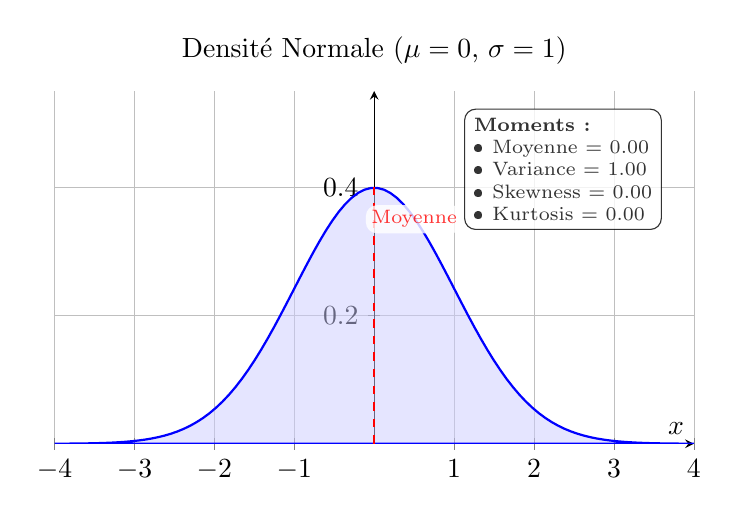
\begin{tikzpicture}
  \begin{axis}[
    width=0.8\textwidth,
    height=0.5\textwidth,
    xlabel={$x$},
    title={Densité Normale ($\mu=0$, $\sigma=1$)},
    grid=both,
    grid style={line width=.1pt, draw=gray!30},
    major grid style={line width=.2pt,draw=gray!50},
    domain=-4:4,
    samples=100,
    enlargelimits=false,
    axis lines=middle,
    xmin=-4, xmax=4,
    ymin=0, ymax=0.55
  ]
 
  % Courbe de densité
  \addplot [thick, color=blue, fill=blue!20, fill opacity=0.5] 
    {1/(sqrt(2*pi))*exp(-x^2/2)} \closedcycle;
 
  % Ligne de la moyenne
  \addplot [red, dashed, thick] coordinates {(0,0) (0,0.4)};
  \node[red, fill=white, font=\scriptsize, rounded corners, inner sep=2pt, opacity=0.8] at (axis cs:0.5,0.35) {Moyenne};
 
  % Boîte de texte avec moments seulement
  \node [draw=black, fill=white, rounded corners, font=\scriptsize, align=left, anchor=north east, opacity=0.8] 
    at (axis description cs:0.95,0.95) { % MODIFIÉ
    \textbf{Moments :}\\
    • Moyenne = 0.00\\
    • Variance = 1.00\\
    • Skewness = 0.00\\
    • Kurtosis = 0.00
    };
    
  \end{axis}
\end{tikzpicture}
\end{center}

La distribution normale est l'archétype de la courbe en cloche. Imaginez une cible : la majorité des flèches touchent le centre, et plus on s'éloigne du centre, moins il y a de chances d'être touché. C'est une distribution parfaitement symétrique, ce qui se traduit par un \textbf{skewness nul (0.00)}. Son pic est ni trop pointu, ni trop plat : c'est notre point de référence, on dit qu'elle est \textbf{mésokurtique}, d'où son kurtosis de \textbf{0.00}. C'est la base de nombreuses analyses statistiques car elle modélise naturellement beaucoup de phénomènes.

\end{examplebox}

\begin{examplebox}[La Distribution Exponentielle (Asymétrique à Droite)]

\begin{center}
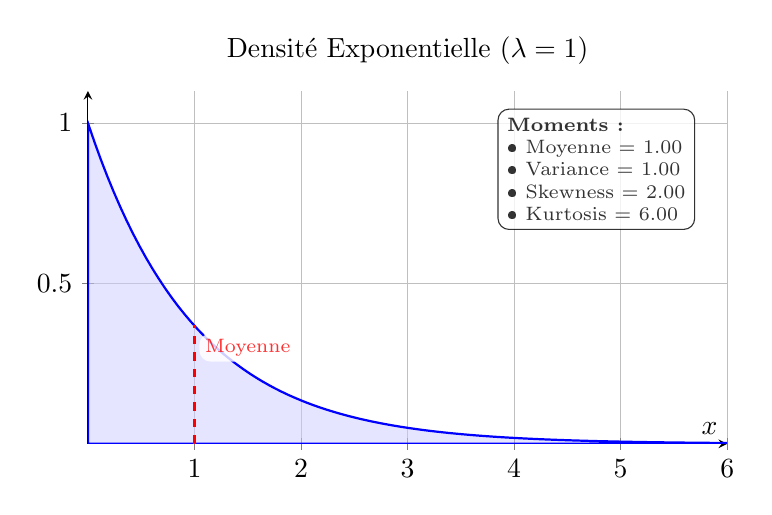
\begin{tikzpicture}
  \begin{axis}[
    width=0.8\textwidth,
    height=0.5\textwidth,
    xlabel={$x$},
    title={Densité Exponentielle ($\lambda=1$)},
    grid=both,
    grid style={line width=.1pt, draw=gray!30},
    major grid style={line width=.2pt,draw=gray!50},
    domain=0:6,
    samples=100,
    enlargelimits=false,
    axis lines=middle,
    xmin=0, xmax=6,
    ymin=0, ymax=1.1
  ]
 
  % Courbe de densité exponentielle
  \addplot [thick, color=blue, fill=blue!20, fill opacity=0.5] 
    {exp(-x)} \closedcycle;
 
  % Ligne de la moyenne
  \addplot [red, dashed, thick] coordinates {(1,0) (1,0.37)};
  \node[red, fill=white, font=\scriptsize, rounded corners, inner sep=2pt, opacity=0.8] at (axis cs:1.5,0.3) {Moyenne};
 
  % Boîte de texte avec moments seulement
  \node [draw=black, fill=white, rounded corners, font=\scriptsize, align=left, anchor=north east, opacity=0.8] 
    at (axis description cs:0.95,0.95) { % MODIFIÉ
    \textbf{Moments :}\\
    • Moyenne = 1.00\\
    • Variance = 1.00\\
    • Skewness = 2.00\\
    • Kurtosis = 6.00
    };
    
  \end{axis}
\end{tikzpicture}
\end{center}

Imaginez le temps d'attente avant un événement rare, comme un appel téléphonique. La plupart du temps, l'appel arrive vite, mais il peut parfois y avoir de longues attentes. C'est exactement ce que modélise la distribution exponentielle : un pic à gauche et une longue queue à droite. Cela se traduit par un \textbf{skewness positif élevé (2.00)}, indiquant une asymétrie marquée. Elle est aussi \textbf{leptokurtique} (\textbf{kurtosis = 6.00}) : son pic est pointu, et la longue queue droite signifie qu'il y a une probabilité non négligeable de valeurs extrêmes.

\end{examplebox}

\begin{examplebox}[La Distribution Uniforme (Platykurtique)]

\begin{center}
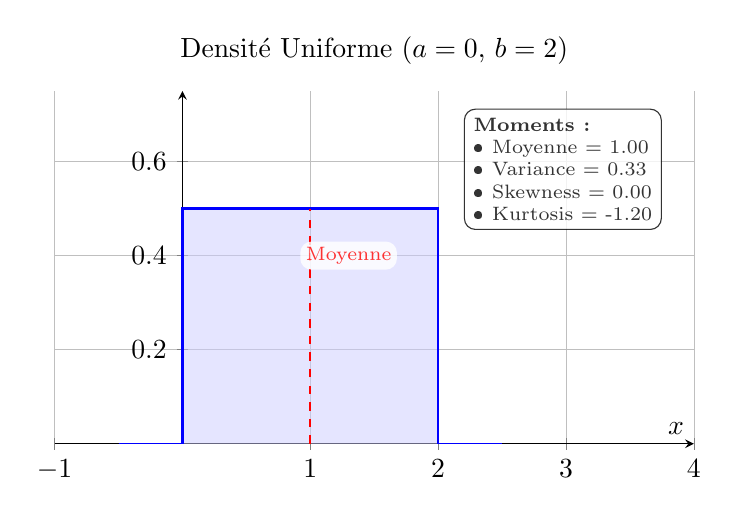
\begin{tikzpicture}
  \begin{axis}[
    width=0.8\textwidth,
    height=0.5\textwidth,
    xlabel={$x$},
    title={Densité Uniforme ($a=0$, $b=2$)},
    grid=both,
    grid style={line width=.1pt, draw=gray!30},
    major grid style={line width=.2pt,draw=gray!50},
    domain=-0.5:2.5,
    samples=100,
    enlargelimits=false,
    axis lines=middle,
    ymin=0,
    ymax=.75,
    xmin=-1, xmax=4
  ]
 
  % Courbe de densité uniforme
  \addplot [thick, color=blue, fill=blue!20, fill opacity=0.5, const plot] 
    coordinates {(-0.5,0) (0,0) (0,0.5) (2,0.5) (2,0) (2.5,0)};
 
  % Ligne de la moyenne
  \addplot [red, dashed, thick] coordinates {(1,0) (1,0.5)};
  \node[red, fill=white, font=\scriptsize, rounded corners, inner sep=2pt, opacity=0.8] at (axis cs:1.3,0.4) {Moyenne};
 
  % Boîte de texte avec moments seulement
  \node [draw=black, fill=white, rounded corners, font=\scriptsize, align=left, anchor=north east, opacity=0.8] 
    at (axis description cs:0.95,0.95) { % MODIFIÉ
    \textbf{Moments :}\\
    • Moyenne = 1.00\\
    • Variance = 0.33\\
    • Skewness = 0.00\\
    • Kurtosis = -1.20
    };
    
  \end{axis}
\end{tikzpicture}
\end{center}

La distribution uniforme, c'est le "tirage au sort parfait" : chaque valeur sur un intervalle a la même chance d'être tirée. Visuellement, c'est un rectangle, donc aucune valeur n'est privilégiée. Elle est symétrique (\textbf{skewness = 0.00}), mais contrairement à la normale, elle est "plate", sans pic central. Cela se traduit par un \textbf{kurtosis négatif (-1.20)}, ce qui signifie qu'elle est \textbf{platykurtique}. Elle est donc très différente des distributions avec un pic central comme la normale.

\end{examplebox}

\begin{examplebox}[La Distribution Log-Normale (Fortement Leptokurtique)]

\begin{center}
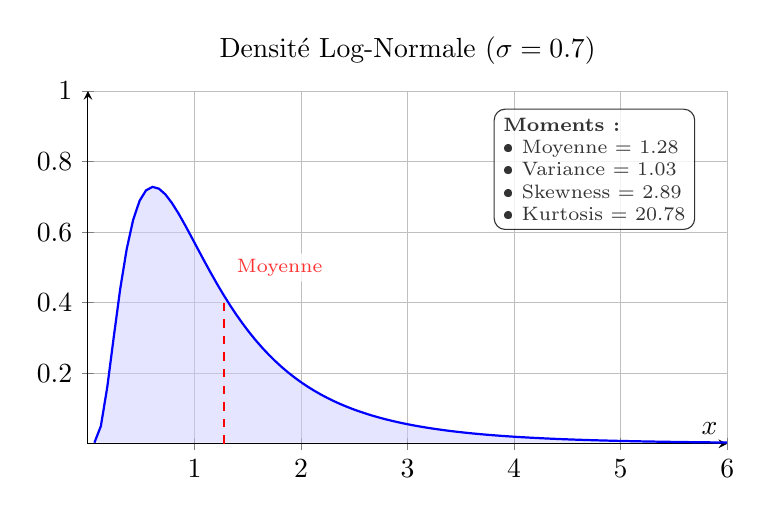
\begin{tikzpicture}
  \begin{axis}[
    width=0.8\textwidth,
    height=0.5\textwidth,
    xlabel={$x$},
    title={Densité Log-Normale ($\sigma=0.7$)},
    grid=both,
    grid style={line width=.1pt, draw=gray!30},
    major grid style={line width=.2pt,draw=gray!50},
    domain=0:6,
    samples=100,
    enlargelimits=false,
    axis lines=middle,
    xmin=0, xmax=6,
    ymin=0, ymax=1
  ]
 
  % Courbe de densité log-normale
  \addplot [thick, color=blue, fill=blue!20, fill opacity=0.5] 
    {1/(x*0.7*sqrt(2*pi))*exp(-(ln(x))^2/(2*0.7^2))};
 
  % Ligne de la moyenne
  \addplot [red, dashed, thick] coordinates {(1.28,0) (1.28,0.4)};
  \node[red, fill=white, font=\scriptsize, rounded corners, inner sep=2pt, opacity=0.8] at (axis cs:1.8,0.5) {Moyenne};
 
  % Boîte de texte avec moments seulement
  \node [draw=black, fill=white, rounded corners, font=\scriptsize, align=left, anchor=north east, opacity=0.8] 
    at (axis description cs:0.95,0.95) { % MODIFIÉ
    \textbf{Moments :}\\
    • Moyenne = 1.28\\
    • Variance = 1.03\\
    • Skewness = 2.89\\
    • Kurtosis = 20.78
    };
    
  \end{axis}
\end{tikzpicture}
\end{center}

La log-normale est une distribution très asymétrique. Imaginez la richesse d'une population : la majorité est modeste, mais il existe une petite proportion de très riches, ce qui "étire" la droite de la courbe. Cela donne un \textbf{skewness très élevé (2.89)}. Elle est extrêmement \textbf{leptokurtique} (\textbf{kurtosis = 20.78}) : un pic très aigu et une queue droite très lourde. Cela signifie qu'il y a un risque élevé de valeurs extrêmement grandes, ce qui la rend très utile pour modéliser des phénomènes avec de rares événements extrêmes.

\end{examplebox}

Nous avons défini les moments d'une \textit{distribution} (moments de population), tels que $\mu = E[X]$ ou $\sigma^2 = E[(X-\mu)^2]$. Ce sont des valeurs théoriques, la "vérité" sous-jacente.

En pratique, nous ne connaissons presque jamais cette "vérité". Nous ne disposons que de données. Notre but est d'utiliser ces données pour \textit{estimer} les moments de la population.

\subsection{Moments d'échantillon (Sample Moments)}

\begin{definitionbox}[Moments d'Échantillon]
Soit $X_1, X_2, \dots, X_n$ un échantillon de $n$ observations.
\begin{itemize}
    \item La \textbf{moyenne d'échantillon} (notre "meilleure estimation" de $\mu$) est :
    $$ \bar{X} = \frac{1}{n} \sum_{i=1}^n X_i $$
    \item La \textbf{variance d'échantillon (non biaisée)} (notre "meilleure estimation" de $\sigma^2$) est :
    $$ s^2 = \frac{1}{n-1} \sum_{i=1}^n (X_i - \bar{X})^2 $$
\end{itemize}
De même, on peut calculer un \textit{skewness d'échantillon} et un \textit{kurtosis d'échantillon} en utilisant $\bar{X}$ et $s$, qui seront nos estimations du vrai skewness et du vrai kurtosis de la population.
\end{definitionbox}

\begin{examplebox}[Application : Contrôle Qualité ]
Imaginez une usine qui produit des sacs de sucre de 1kg.
\begin{itemize}
    \item \textbf{Population :} L'infinité de tous les sacs de sucre que la machine produira.
    \item \textbf{Moment de population (inconnu) :} Le poids moyen \textit{réel} $\mu$ que la machine verse, et la variance \textit{réelle} $\sigma^2$ (sa constance).
    \item \textbf{Problème :} Nous ne pouvons pas peser tous les sacs !
    \item \textbf{Solution :} Nous prélevons un \textbf{échantillon} de $n=10$ sacs.
    
    Nous les pesons : $\{ 1002g, 998g, 1001g, 995g, 1003g, 1000g, 997g, 1005g, 999g, 1000g \}$.
    
    \item \textbf{Calcul des moments d'échantillon :}
    \begin{itemize}
        \item $\bar{X} = (1002 + 998 + \dots + 1000) / 10 = 1000g$.
        \item $s^2 = \frac{1}{10-1} \left( (1002-1000)^2 + (998-1000)^2 + \dots \right) = 7.33 g^2$.
    \end{itemize}
    \item \textbf{Conclusion :} Notre meilleure estimation est que la machine est bien réglée sur $\mu = 1000g$. L'écart-type de notre échantillon est $s = \sqrt{7.33} \approx 2.7g$. Nous pouvons utiliser cela pour affirmer, par exemple, que 95\% des sacs se situent probablement entre $1000 \pm 2s$ (si la distribution est normale).
\end{itemize}
\end{examplebox}

\begin{remarquebox}[L'Intuition du "$n-1$"]
Pourquoi diviser par $n-1$ pour la variance ? C'est la \textbf{correction de Bessel}.

Imaginez un échantillon de 1 seule personne ($n=1$). Sa taille est 170cm.
\begin{itemize}
    \item Quelle est la moyenne de l'échantillon ? $\bar{X} = 170$ cm.
    \item Quelle est la variance de l'échantillon ? $\sum (X_i - \bar{X})^2 = (170 - 170)^2 = 0$.
    \item Si on divisait par $n=1$, on estimerait que la variance de la population est 0. C'est absurde ! Cela voudrait dire que tout le monde mesure 170cm.
\end{itemize}
En divisant par $n-1$ (donc $1-1=0$), la formule devient $0/0$ (indéfinie), ce qui nous dit à juste titre : "Je ne peux pas estimer la dispersion avec une seule personne."

\textbf{Intuition plus générale :} Nous "perdons un degré de liberté". Pour calculer la variance, nous avons besoin de connaître la moyenne. Mais nous ne connaissons pas la vraie moyenne $\mu$. Nous devons donc utiliser $\bar{X}$, une \textit{estimation}. Le fait d'utiliser une estimation calculée \textit{à partir de ce même échantillon} introduit un léger biais (nos données sont, par définition, centrées sur $\bar{X}$). Diviser par $n-1$ au lieu de $n$ "gonfle" légèrement le résultat pour compenser ce biais.
\end{remarquebox}

\subsection{Fonctions génératrices des moments (MGF)}

\begin{definitionbox}[Fonction Génératrice des Moments (MGF)]
La \textbf{fonction génératrice des moments} (MGF) d'une variable aléatoire $X$, notée $M_X(t)$, est définie comme :
$$ M_X(t) = E[e^{tX}] $$
\end{definitionbox}

\begin{intuitionbox}[L'ADN, le Code-Barres, ou le Fichier .zip]
Ce concept est abstrait, alors utilisons des analogies :

\textbf{Analogie 1 : L'ADN ou l'Empreinte Digitale}
\begin{itemize}
    \item La MGF est l'**empreinte digitale unique** d'une distribution.
    \item Elle "compresse" \textit{toutes} les informations sur votre distribution (moyenne, variance, skewness, kurtosis, etc.) en une seule, unique fonction.
    \item Si deux distributions ont la même MGF, elles sont identiques. C'est la \textbf{propriété d'unicité}.
\end{itemize}

\textbf{Analogie 2 : Le Code-Barres}
\begin{itemize}
    \item Pensez à une distribution (ex: Loi Normale) comme à un produit au supermarché.
    \item La MGF, $M_X(t)$, est son **code-barres unique**.
    \item Le processus de "génération de moments" (que nous verrons ci-dessous) est le \textbf{scanner}.
    \item En scannant le code-barres ($M_X(t)$), vous pouvez obtenir n'importe quelle information :
        \item Scan 1 ($M_X'(0)$) $\to$ vous donne le prix ($E[X]$).
        \item Scan 2 ($M_X''(0)$) $\to$ vous donne le poids ($E[X^2]$).
        \item Scan 3 ($M_X'''(0)$) $\to$ vous donne le pays d'origine ($E[X^3]$).
\end{itemize}

\textbf{Pourquoi $e^{tX}$ ?}
La "magie" vient du développement en série de Taylor de $e^x$:
$$ e^{tX} = 1 + (tX) + \frac{(tX)^2}{2!} + \frac{(tX)^3}{3!} + \dots $$
Quand on prend l'espérance, $E[\cdot]$, les puissances de $X$ (c'est-à-dire $X, X^2, X^3\dots$) apparaissent. Ce sont les moments ! La MGF "stocke" tous ces moments en les organisant comme coefficients d'un polynôme infini en $t$.
\end{intuitionbox}

\subsection{Génération des moments via les MGF}

\begin{theorembox}[Moments par Dérivation]
Si la MGF $M_X(t)$ existe, alors le $m$-ième moment non centré $E[X^m]$ est la $m$-ième dérivée de $M_X(t)$, évaluée en $t=0$ :
$$ E[X^m] = \frac{d^m}{dt^m} M_X(t) \bigg|_{t=0} = M_X^{(m)}(0) $$
\end{theorembox}

\begin{examplebox}[Application : La Loi de Poisson]
Une loi de Poisson modélise le nombre d'événements (ex: appels à un centre d'appels) par heure. Soit $X \sim \text{Poisson}(\lambda)$, où $\lambda$ est le nombre moyen d'appels.

La MGF (l'ADN) d'une loi de Poisson est (on l'admet) :
$$ M_X(t) = e^{\lambda(e^t - 1)} $$

Utilisons notre "scanner" (les dérivées) pour trouver les moments.

\textbf{1. Trouver la Moyenne $E[X]$ :}
On dérive une fois (règle de la chaîne) :
$$ M_X'(t) = \frac{d}{dt} \left( e^{\lambda(e^t - 1)} \right) = \underbrace{e^{\lambda(e^t - 1)}}_{\text{répète}} \cdot \underbrace{(\lambda e^t)}_{\text{dérivée interne}} $$
Maintenant, on évalue en $t=0$ :
$$ E[X] = M_X'(0) = e^{\lambda(e^0 - 1)} \cdot (\lambda e^0) = e^{\lambda(1 - 1)} \cdot (\lambda \cdot 1) = e^0 \cdot \lambda = 1 \cdot \lambda = \lambda $$
\textbf{Résultat :} La moyenne est $\lambda$, ce qui est la définition même du paramètre de la loi de Poisson. Parfait.

\textbf{2. Trouver $E[X^2]$ (pour la variance) :}
On dérive une seconde fois (règle du produit sur $M_X'(t) = (\lambda e^t) \cdot (e^{\lambda(e^t - 1)})$) :
$$ M_X''(t) = \underbrace{(\lambda e^t)}_{\text{dérivée de u}} \cdot \underbrace{(e^{\lambda(e^t - 1)})}_{\text{v}} + \underbrace{(\lambda e^t)}_{\text{u}} \cdot \underbrace{(e^{\lambda(e^t - 1)} \cdot \lambda e^t)}_{\text{dérivée de v}} $$
Maintenant, on évalue en $t=0$ (tous les $e^0$ deviennent 1) :
$$ E[X^2] = M_X''(0) = (\lambda \cdot 1) \cdot (e^{\lambda(1-1)}) + (\lambda \cdot 1) \cdot (e^{\lambda(1-1)} \cdot \lambda \cdot 1) $$
$$ E[X^2] = (\lambda) \cdot (e^0) + (\lambda) \cdot (e^0 \cdot \lambda) = \lambda \cdot 1 + \lambda \cdot (1 \cdot \lambda) = \lambda + \lambda^2 $$

\textbf{3. Trouver la Variance $\text{Var}(X)$ :}
$\text{Var}(X) = E[X^2] - (E[X])^2 = (\lambda + \lambda^2) - (\lambda)^2 = \lambda$
\textbf{Résultat :} Nous avons prouvé par les MGF que pour une loi de Poisson, $\text{Moyenne} = \text{Variance} = \lambda$. C'est une propriété fondamentale de cette loi.
\end{examplebox}

\subsection{Sommes de variables aléatoires indépendantes via les MGF}

C'est la super-puissance des MGF.

\begin{theorembox}[MGF d'une Somme]
Soient $X$ et $Y$ deux variables aléatoires \textbf{indépendantes}. Soit $S = X + Y$. Alors la MGF de $S$ est le produit des MGF individuelles :
$$ M_S(t) = M_{X+Y}(t) = M_X(t) \cdot M_Y(t) $$
\end{theorembox}

\begin{intuitionbox}[La Magie de l'Exponentielle]
Pourquoi est-ce vrai ? $M_{X+Y}(t) = E[e^{t(X+Y)}] = E[e^{tX} \cdot e^{tY}]$.
Parce que $X$ et $Y$ sont indépendantes, $E[f(X)g(Y)] = E[f(X)]E[g(Y)]$.
Donc, $E[e^{tX} \cdot e^{tY}] = E[e^{tX}] \cdot E[e^{tY}] = M_X(t) \cdot M_Y(t)$.

Les MGF transforment une opération analytiquement horrible (la "convolution" de densités) en une simple multiplication algébrique.
\end{intuitionbox}

\begin{examplebox}[Application : Portefeuille d'Actifs ou Tailles Humaines]
C'est l'un des théorèmes les plus importants des statistiques.
\textbf{Problème :} Soit $X$ la taille d'un homme, $X \sim N(\mu_X, \sigma_X^2)$. Soit $Y$ la taille d'une femme, $Y \sim N(\mu_Y, \sigma_Y^2)$. Si on les choisit au hasard, quelle est la loi de la somme de leurs tailles $S = X+Y$ ?

\begin{enumerate}
    \item \textbf{ADN de $X$} : La MGF d'une loi Normale $N(\mu, \sigma^2)$ est $M(t) = \exp(\mu t + \frac{1}{2}\sigma^2 t^2)$.
    \item \textbf{ADN de $X$ et $Y$} :
    $M_X(t) = \exp(\mu_X t + \frac{1}{2}\sigma_X^2 t^2)$
    $M_Y(t) = \exp(\mu_Y t + \frac{1}{2}\sigma_Y^2 t^2)$
    
    \item \textbf{ADN de $S = X+Y$} (on multiplie) :
    $M_S(t) = M_X(t) \cdot M_Y(t) = \exp(\mu_X t + \frac{1}{2}\sigma_X^2 t^2) \cdot \exp(\mu_Y t + \frac{1}{2}\sigma_Y^2 t^2)$
    
    \item \textbf{Simplification} (en additionnant les exposants) :
    $M_S(t) = \exp\left( (\mu_X t + \mu_Y t) + (\frac{1}{2}\sigma_X^2 t^2 + \frac{1}{2}\sigma_Y^2 t^2) \right)$
    $M_S(t) = \exp\left( (\mu_X + \mu_Y)t + \frac{1}{2}(\sigma_X^2 + \sigma_Y^2)t^2 \right)$
    
    \item \textbf{Conclusion (par Unicité)} :
    Regardez cet ADN ! C'est l'ADN d'une loi Normale !
    Le nouveau $\mu$ est $(\mu_X + \mu_Y)$.
    La nouvelle $\sigma^2$ est $(\sigma_X^2 + \sigma_Y^2)$.
\end{enumerate}

\textbf{Résultat :} Nous avons prouvé que \textbf{la somme de deux Normales indépendantes est une nouvelle Normale}.
Si $X \sim N(175cm, 7^2)$ et $Y \sim N(165cm, 6^2)$, alors $S \sim N(340cm, 7^2 + 6^2 = 85)$.
Notez que les écarts-types \textit{ne s'additionnent pas} ($\sqrt{85} \approx 9.2 \ne 7+6$). Ce sont les variances qui s'additionnent.
\end{examplebox}